\documentclass[a4paper,14pt]{article}

\usepackage[12pt]{extsizes}
\usepackage{cmap}					% поиск в PDF
\usepackage{mathtext} 				% русские буквы в формулах
\usepackage[T2A]{fontenc}			% кодировка
\usepackage[utf8]{inputenc}			% кодировка исходного текста
\usepackage[english,russian]{babel}	% локализация и переносы
\usepackage{graphicx}
\usepackage{geometry}
\usepackage{amsmath}
\usepackage{amssymb}
\usepackage[table]{xcolor}
\setlength\extrarowheight{2pt}


\geometry{verbose, a4paper, tmargin=2cm, bmargin=2cm, lmargin=2cm, rmargin=2cm}
\author{Vysotsky Maxim}
\title{Отчёт}
\date{2025}

\begin{document}
	\begin{titlepage}
		\begin{center}
			{Министерство науки и высшего образования Российской Федерации
				НОВОСИБИРСКИЙ НАЦИОНАЛЬНЫЙ ИССЛЕДОВАТЕЛЬСКИЙ
				ГОСУДАРСТВЕННЫЙ УНИВЕРСИТЕТ (НГУ)}
		\end{center}
		\begin{center}
			{Физический факультет}
		\end{center}
		\begin{center}
			{Кафедра общей физики}
		\end{center}
		
		
		\vspace{7cm}
		{
			\begin{center}
				{\bf Лабораторная работа №3.4}\\
			Определение коэффициента поверхностного
натяжения жидкостей волновыс методом.
			\end{center}
		}
		\vspace{2cm}
		\begin{flushright}
			{Руководитель:\\ Ассистент\\
				Художитков В. Э.\\
                Старший преподаватель \\
                Кравцова А. Ю.\\
				Работу выполнил:\\
				Высоцкий М. Ю.\\
				\vspace{0.2cm}
				гр. 24301}
		\end{flushright}
		\vspace{3cm}
		\begin{center}
			Новосибирск, 2025
		\end{center}
	\end{titlepage}


\section{Теоретическое введение}
\hspace{\parindent}\textbf{Цель работы:} измерение коэффициента поверхностного
натяжения дистиллированной воды и ряда других жидкостей;
определение зависимости коэффициента поверхностного
натяжения от концентрации примесей; оценка размеров молекул
жидкости.

\textbf{Оборудование:} генератор переменного напряжения,
импульсный источник света, вибратор, кювета, набор
исследуемых жидкостей.

\textbf{Коэффициент поверхностного натяжения} - работа, которую надо затратить, чтобы изотермически и  квазистатически увеличить площадь поверхности жидкости
на единицу при сохранении ее объема неизменным.

$$
\sigma= \frac{F}{2l}
$$
$$
[\sigma] = \frac{Н}{м}
$$

Кривизна поверхности:
$$
K = \frac{1}{R_1} + \frac{1}{R_2}
$$

Формула Лапласа:
$$
\sigma K = \sigma \left(\frac{1}{R_1} + \frac{1}{R_2}\right) = P_В - P_Н
$$

Рабочая формула:
$$
\sigma = \frac{\rho\lambda^2}{4\pi^2}(2\pi f^2\lambda-g)
$$
$\rho$ - плотность жидкости, $\lambda$ - длина волны, $g$ - ускорение свободного падения, $f = 1/T = с/\lambda$, $с$ - скорость волны.

Схема установки:
\begin{figure}[!ht]
    \centering
    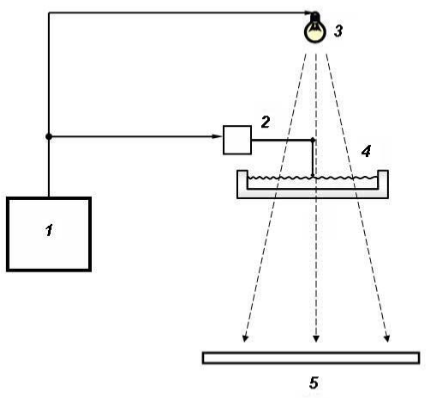
\includegraphics[scale=0.4]{scheme.png}
    \caption{Cхема установки: 1 – генератор переменного тока; 2 – вибратор
(генератор поверхностных волн); 3 – импульсный источник света; 4 –
прозрачная кювета с исследуемой жидкостью; 5 – экран} 
\end{figure}

\clearpage

\subsection{Ход эксперимента}
\hspace{\parindent}Данные, полученные для дистиллированной воды и раствора глицерина 10\%-40\%, приведены ниже. Также в ходе работы был получен коэффициент увеличения оптики $\kappa=\frac{1}{4}$.

\begin{table}[!ht]
    \centering
    \begin{tabular}{|l|l|l|l|}
    \hline
        $\nu$, Гц & $\lambda$, см & $\kappa*\lambda$, м & $\sigma$, Н/м \\ \hline
        50 & 1,5 & 0,060 & 85,07 \\ \hline
        60 & 1,4 & 0,056 & 99,88 \\ \hline
        70 & 1,2 & 0,048 & 85,71 \\ \hline
        80 & 1,2 & 0,048 & 112,12 \\ \hline
        90 & 1 & 0,040 & 82,14 \\ \hline
        100 & 0,9 & 0,036 & 73,96 \\ \hline
        110 & 0,9 & 0,036 & 89,57 \\ \hline
    \end{tabular}
    \caption{Данные для воды.}
\end{table}

\begin{table}[!ht]
    \centering
    \begin{tabular}{|l|l|l|l|}
    \hline
        $\nu$, Гц & $\lambda$, см & $\kappa*\lambda$, м & $\sigma$, Н/м \\ \hline
        25 & 2,2 & 0,088 & 65,86 \\ \hline
        30 & 2,2 & 0,088 & 95,70 \\ \hline
        40 & 1,9 & 0,076 & 110,38 \\ \hline
        50 & 1,4 & 0,056 & 69,12 \\ \hline
        60 & 1,4 & 0,056 & 99,88 \\ \hline
        70 & 1 & 0,040 & 49,53 \\ \hline
        80 & 1 & 0,040 & 64,82 \\ \hline
    \end{tabular}
    \caption{Данные для глицерина 10\%.}
\end{table}

\begin{table}[!ht]
    \centering
    \begin{tabular}{|l|l|l|l|}
    \hline
        $\nu$, Гц & $\lambda$, см & $\kappa*\lambda$, м & $\sigma$, Н/м \\ \hline
        15 & 2,4 & 0,096 & 29,36 \\ \hline
        30 & 1,8 & 0,072 & 52,18 \\ \hline
        35 & 1,6 & 0,064 & 50,10 \\ \hline
        40 & 1,5 & 0,060 & 54,12 \\ \hline
        60 & 1,1 & 0,044 & 48,34 \\ \hline
        70 & 1 & 0,040 & 49,53 \\ \hline
    \end{tabular}
    \caption{Данные для глицерина 20\%.}
\end{table}

\clearpage

\begin{table}[!ht]
    \centering
    \begin{tabular}{|l|l|l|l|}
    \hline
        $\nu$, Гц & $\lambda$, см & $\kappa*\lambda$, м & $\sigma$, Н/м \\ \hline
        25 & 2,4 & 0,096 & 85,71 \\ \hline
        30 & 2,1 & 0,084 & 83,15 \\ \hline
        35 & 1,6 & 0,064 & 50,10 \\ \hline
        40 & 1,5 & 0,060 & 54,12 \\ \hline
        60 & 1,2 & 0,048 & 62,81 \\ \hline
        70 & 1 & 0,040 & 49,53 \\ \hline
    \end{tabular}
    \caption{Данные для глицерина 30\%.}
\end{table}

\begin{table}[!ht]
    \centering
    \begin{tabular}{|l|l|l|l|}
    \hline
        $\nu$, Гц & $\lambda$, см & $\kappa*\lambda$, м & $\sigma$, Н/м \\ \hline
        25 & 2 & 0,080 & 49,33 \\ \hline
        30 & 1,9 & 0,076 & 61,45 \\ \hline
        35 & 1,7 & 0,068 & 60,16 \\ \hline
        40 & 1,5 & 0,060 & 54,12 \\ \hline
        60 & 1,1 & 0,044 & 48,34 \\ \hline
        70 & 0,9 & 0,036 & 36,07 \\ \hline
    \end{tabular}
    \caption{Данные для глицерина 40\%.}
\end{table}
Средние значения коэффициента поверхностного натяжения для дистиллированной воды, раствора глицерина 10\%-40\% соответственно: 
$$
\sigma_{воды} = 89,78*10^{-3} \frac{Н}{м}
$$

$$
\sigma_{глиц10\%} = 79,32*10^{-3} \frac{Н}{м}
$$

$$
\sigma_{глиц20\%} = 47,27*10^{-3} \frac{Н}{м}
$$

$$
\sigma_{глиц30\%} = 64,24*10^{-3} \frac{Н}{м}
$$

$$
\sigma_{глиц40\%} = 51,58*10^{-3} \frac{Н}{м}
$$

\clearpage

Также был получен график зависимости коэффициента поверхностного натяжения от концентрации раствора глицерина.

\begin{figure}[!ht]
    \centering
    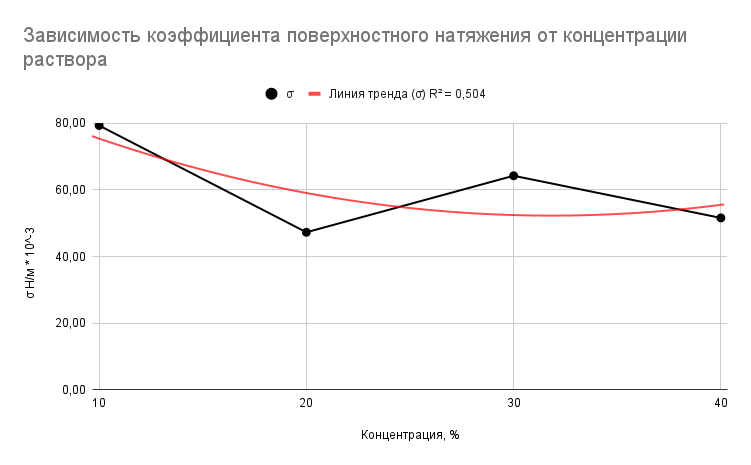
\includegraphics[scale=0.6]{sigma1.png}
    \caption{Зависимость коэффициента поверхностного натяжения от концентрации раствора глицерина} 
\end{figure}

\section{Вывод}
\hspace{\parindent}Как видно из графика выше, данные для 20\%-процентного, 30\%-процентного, 40\%-процентного глицерина оказались не совсем корректными. Они оказались того же порядка, но выше по значению, и зависимость должна быть гиперболической, то есть убывать. В целом, линия тренда показывает именно такю зависимость. Такая ошибка могла быть допущена в силу того, что нам пришлось самостоятельно замешивать растворы глицерина (а именно 20\% и 40\%) и не во всех сериях заливался одинаковый объем вещества в кювету. Возможно, мы допустили ошибку при смешивании, либо 30\% раствор был изначально неверно замешан. 

Теоретически, с увеличением содержания глицерина, коэффициент поверхностного натяжения уменьшается. 
\end{document}
